
%%%%    IMPORTS 2 BASE    %%%%


\documentclass[hidelinks, french, oneside]{article}
\usepackage[utf8]{inputenc}
\usepackage[T1]{fontenc}

% pour le mise en page
\usepackage[a4paper, total={6.5in, 10in}]{geometry}
\usepackage{fontsize} \changefontsize[13]{10}		
\usepackage{xcolor}

% mathsymbole
\usepackage{amsmath, amssymb,stmaryrd}
\usepackage{wasysym}[mathcal] % a quoi sert le [mathcal] ?
\usepackage{nicefrac, units} % fraction pour text mode / unité

% TBD
\usepackage{mathcomp}
\usepackage{mathrsfs} % pour \mathscr a priori

% pour les belles fonts
\usepackage{amsfonts}
\DeclareMathAlphabet{\mathpzc}{OT1}{pzc}{m}{it}
%\usepackage{euscript}[mathcal]
%\usepackage{rsfso}
\usepackage{bbm}	 % mathbb étendu

% pour les hyprlien / cross-ref
\usepackage{hyperref, cleveref}
%\namecref{sec:label}

%pour les figures
\usepackage{graphicx} \usepackage{wrapfig, floatrow}
%\usepackage{subcaption} % surement useless, parsk floatrow-like 

% pour les beaux tableaux
\usepackage{multirow}

% pour des matrices infernales
\usepackage{easybmat}

% pour les citations (aucune idées de comment ca marche)
\usepackage{csquotes}



%%%%    RACCOURCIS    %%%%


% bb / cal / frak
\newcommand{\N}{\mathbb{N}}
\newcommand{\Z}{\mathbb{Z}}             % Note pour homo pour les updates
\newcommand{\Q}{\mathbb{Q}}
\newcommand{\R}{\mathbb{R}}
\newcommand{\C}{\mathbb{C}}
\newcommand{\K}{\mathbb{K}}
\renewcommand{\k}{\Bbbk}
\newcommand{\U}{\mathbb{U}}
\renewcommand{\u}{\text{U}}
\newcommand{\A}{\mathbb{A}}
\newcommand{\T}{\mathscr{T}}
\newcommand{\I}{\mathbb{I}}
\newcommand{\one}{\mathbbm{1}}
%\renewcommand{\S}{\mathfrak{S}}
\renewcommand{\S}{\mathbb{S}}

% arrows
\newcommand{\lr}{\longrightarrow}
\newcommand{\Lr}{\Longrightarrow}
%\renewcommand{\ll}{\longleftarrow}
\newcommand{\Ll}{\Longleftarrow}
\newcommand{\llr}{\longleftrightarrowr}
\newcommand{\Llr}{\Longleftrightarrow}

% espaces
\newcommand{\matk}{\mathpzc{M}_n(\mathbb{K})}
\newcommand{\matr}{\mathpzc{M}_n(\mathbb{R})}

% fonctions
\newcommand{\Arccos}{\text{Arccos}} 
\newcommand{\Arcsin}{\text{Arcsin}} 
\newcommand{\Arctan}{\text{Arctan}} 
\newcommand{\Argch}{\text{Argch}}       
\newcommand{\Argsh}{\text{Argsh}}

\newcommand{\congu}[1]{\overline{#1}}
\newcommand{\argmin}[1]{\underset{#1}{\text{argmin}}}
\newcommand{\argmax}[1]{\underset{#1}{\text{argmax}}}

\newcommand{\pgcd}{\text{pgcd}}
\newcommand{\PGCD}{\text{PGCD}}
\newcommand{\ppmc}{\text{ppcm}}
\newcommand{\sign}{\text{sign}}

\newcommand{\sgn}{\text{sgn}}
%\newcommand{\deg}{\text{deg}}
\newcommand{\ord}{\text{ord}}
\newcommand{\rot}{\text{rot}}

%\renewcommand{\det}{\text{det}}
\newcommand{\tr}{\text{tr}}
\newcommand{\rg}{\text{rg}}
\newcommand{\Co}{\text{com}}
\newcommand{\codim}{\text{codim}}

%espaces
%\renewcommand{\Vec}{\text{Vec}}
\newcommand{\im}{\text{Im}}
\newcommand{\Ker}{\text{Ker}}
\newcommand{\Ann}{\text{Ann}}
\newcommand{\Sp}{\text{Sp}} 
\newcommand{\GL}{\text{GL}}
\newcommand{\SL}{\text{SL}}
\newcommand{\SO}{\text{SO}}
\newcommand{\SU}{\text{SU}}
%\renewcommand{\div}{\text{div}}

\newcommand{\Aff}{\text{Aff}}
\newcommand{\HT}{\text{HT}}
\newcommand{\GA}{\text{GA}}

% spé proba
\newcommand{\esp}[2][]{\mathbb{E}_{#1}\left[\, #2\, \right]}
\newcommand{\var}[2][]{\mathbb{V}_{#1}\left[\, #2\, \right]}
%\newcommand{\Var}{\mathbb{V}}%\text{ar}}

% plus jolie
\renewcommand{\O}{\varnothing}
\renewcommand{\epsilon}{\varepsilon}
\renewcommand{\subsetneq}{\varsubsetneq}
\renewcommand{\leq}{\leqslant}
\renewcommand{\geq}{\geqslant}
\renewcommand{\limsup}{\varlimsup}
\renewcommand{\liminf}{\varliminf}

% autre
\newcommand{\defeq}{:=}
\renewcommand{\bf}[1]{\boldsymbol{#1}}
\renewcommand{\AC}{\sim}
\newcommand{\para}{\sslash}


% latin
\newcommand{\etal}{\textit{et al.}}
\newcommand{\etc}{\textit{etc.}}
\newcommand{\apriori}{\textit{a priori}}
\newcommand{\afortiori}{\textit{a fortiori}}
\newcommand{\acontrario}{\textit{a contrario}}
\newcommand{\infine}{\textit{in fine}}
\newcommand{\ie}{\textit{i.e.}}
\newcommand{\eg}{\textit{e.g.}}

% tmp
\newcommand{\phaset}{\Phi_{\text{tot}}}
\newcommand{\phased}{\Phi_{\text{dyn}}}
\newcommand{\phaseg}{\Phi_{\text{geo}}}



%%%%    ENONCES (PROP, DEF, RQ)    %%%%


\usepackage{amsthm}

% les styles
\newtheoremstyle{enonce}{0pt}{25pt}{}{}{\scshape}{\quad ---\quad }{0em}{}
\newtheoremstyle{special}{0pt}{25pt}{}{}{\scshape}{\quad ---\quad }{0em}{\thmnote{#3}}
\newtheoremstyle{rqlike}{0pt}{25pt}{\itshape}{}{\scshape}{\quad ---\quad}{0em}{}
\newtheoremstyle{exo}{0pt}{25pt}{\color{blue}}{}{\scshape\color{blue}}{: \newline}{0em}{}

% énoncés classiques
\theoremstyle{enonce}
\newtheorem{definition}{Définition}
\newtheorem{proposition}{Proposition}
\newtheorem{propriete}{Propriété}
\newtheorem{propricarac}[propriete]{Propriété Caractéristique}
\newtheorem{lemme}{Lemme}
\newtheorem{theoreme}{Théorème}[section]
\newtheorem{theodef}[theoreme]{Théorème et Définition}
\newtheorem{corollaire}{\qquad Corollaire}[theoreme]

% énoncé type
\theoremstyle{special}
\newtheorem{enonce}{}

% énoncé numérotation-less
\theoremstyle{rqlike}
\newtheorem*{remarque}{\qquad Remarque}
\newtheorem*{rappel}{\qquad Rappel}
\newtheorem*{exemple}{\qquad Exemple}

\theoremstyle{exo}
\newtheorem{exercice}{Exercice}

% pour cref aux enoncés
\crefname{definition}{définition}{Définition}
\crefname{proposition}{proposition}{Proposition}
\crefname{propriete}{propriété}{Propriété}
\crefname{lemme}{lemme}{Lemme}
\crefname{theoreme}{théorème}{Théorème}
\crefname{corollaire}{corollaire}{Corollaire} 

\crefname{remarque}{remarque}{Remarque}
\crefname{rappel}{rappel}{Rappel}
\crefname{exemple}{exemple}{Exemple}

\crefname{exercice}{exercice}{Exercice}

% espace démo  (pas convaincu)
\definecolor{mygray}{gray}{0.3}
\newtheoremstyle{demo}{8pt}{0pt}{\color{mygray}}{}{\itshape\color{mygray}}{\newline\newline}{0em}{}

\theoremstyle{demo}
\newtheorem*{demo}{\qquad\qquad\qquad\rule{3.5cm}{0.4pt}\qquad\quad Démonstration\qquad\quad \rule{3.5cm}{0.4pt}}
%\begin{center}\rule{8cm}{0.4pt}\end{center}



%%%%    PROG N PLOT    %%%%


% Prog

%\usepackage{fancyvrb} % pour le lore, mais useless AF
\usepackage{listings} 
\usepackage{pythontex}	% surement une dingz, à approfondire

% preset
\definecolor{codeblack}{gray}{0.2}
\definecolor{codegreen}{rgb}{0,0.6,0}
\definecolor{codegray}{gray}{0.5}
\definecolor{codepurple}{rgb}{0.58,0,0.82}
\definecolor{backcolour}{rgb}{0.98,0.98,0.95}

\lstdefinestyle{mystyle}{
backgroundcolor=\color{backcolour},   
commentstyle=\color{codegray},
keywordstyle=\color{orange},
numberstyle=\tiny\color{codegray},
stringstyle=\color{codegreen},
basicstyle=\color{codeblack}\ttfamily\footnotesize,
breakatwhitespace=false,         
breaklines=true,                 
captionpos=b,
abovecaptionskip=12,
belowcaptionskip=18,
keepspaces=true,                 
numbers=left,                    
numbersep=5pt,                  
showspaces=false,                
showstringspaces=false,
showtabs=false,                  
tabsize=2,
frame=single,
rulecolor=\color{lightgray}}
\lstset{style=mystyle}


% Plot

% pour dessins et les diagrams
\usepackage{tikz, tikz-cd, tkz-euclide}
\usepackage{scalerel, pict2e}
\usetikzlibrary{calc, patterns, shapes.arrows, arrows.meta, shadows, external} 

% pour les maxis plots
\usepackage{pgfplots}
\pgfplotsset{compat=newest, scaled y ticks=false}
\usepgfplotslibrary{groupplots, dateplot, statistics, fillbetween}

\tikzstyle{every node}=[font=\scriptsize]
\pgfplotsset{standard/.style={width=8cm,
	height=3cm,
	compat=1.18,
	trig format=rad,
	enlargelimits,
	axis x line=middle,
	axis y line=middle,
	enlarge x limits=0.15,
	enlarge y limits=0.15,
	every axis x label/.style={footnotesize, at={(current axis.right of origin)},anchor=north west},
	every axis y label/.style={footnotesize, at={(current axis.above origin)},anchor=south east},
	scale only axis=true}}
	
	
	
	%%%%    CAPTIONS 2 FIGURES    %%%%
	
	
	% set up des captions figures (extrêmement BG)
	
	% pos et séparateur générale
	\captionsetup{justification=centering}
	\DeclareCaptionLabelSeparator{custom}{\, ---\, }
	
	% spécial figure
	\DeclareCaptionLabelFormat{customfig}{\textit{fig. #2}}
	\DeclareCaptionFormat{customfig}{#1#2#3}
	%\DeclareCaptionFont{customfig}{\itshape} %marche pas jsppk
	\renewcommand{\thefigure}{\arabic{section}.\arabic{figure}}
	\captionsetup[figure]{labelformat=customfig, labelsep=custom}
	
	% spécial code (listings)
	\DeclareCaptionLabelFormat{customcode}{\textit{code \arabic{section}.#2}}
	\DeclareCaptionFormat{customcode}{#1#2#3}
	%\renewcommand{\thelstlisting}{\arabic{section}.\arabic{lstlisting}}
	\captionsetup[lstlisting]{labelformat=customcode, labelsep=custom}
	
	
	
	%%%%    TABLES/REF  &  HAUT/BAS DE PAGES    %%%%
	
	
	% nom des tables et références
	
	\renewcommand{\contentsname}{\begin{center}\textsc{Tables des Matrières}\end{center}}
	\renewcommand{\listfigurename}{\begin{center}\textsc{Table des Figures}\end{center}}
	\renewcommand{\lstlistlistingname}{\begin{center}\textsc{Table des Codes}\end{center}}
	\renewcommand{\refname}{\begin{center}\textsc{Références}\end{center}}
	
	% bas/haut de page (à optimiser à l'occas')
	
	\usepackage{fancyhdr}
	\pagestyle{fancy}                       
	\fancyhf{}
	\renewcommand{\headrulewidth}{0pt}
	\cfoot{\thepage}
	
	%version2réjane  :
	%\usepackage{eso-pic}
	%\renewcommand\headrulewidth{1pt}
	%\fancyhead[L]{\includegraphics[width=3cm]{logo_lr.png}}
	%\fancyhead[R]{\includegraphics[width=1cm]{logo_sdis17.png}}
	%\setlength{\headsep}{45pt}
	
	
	
	%%%%    SECTIONS ET TOC    %%%%
	
	
	% génération des sections
	
\usepackage[loadonly, toctitles, clearempty, newparttoc]{titlesec}

% liste des sections
\titleclass{\part}[0]{top} % 0 = niveau de section
\titleclass{\section}{straight}[\part]
\titleclass{\subsection}{straight}[\section]
\titleclass{\subsubsection}{straight}[\subsection]

% génère les numérotations avec format
%\newcounter{part}
\renewcommand{\thepart}{\Roman{part}}
%\newcounter{section}
\renewcommand{\thesection}{\Roman{section}}
%\newcounter{subsection}
\renewcommand{\thesubsection}{\arabic{section}.\arabic{subsection}}
%\newcounter{subsubsection}
\renewcommand{\thesubsubsection}{\arabic{section}.\arabic{subsection}.\arabic{subsubsection}}

% formatage
\titleformat{\part}[display]{\bfseries\scshape\Large}{\centering \rule{3.5cm}{0.4pt}\qquad Chapitre\quad \thepart \qquad \rule{3.5cm}{0.4pt}}{15pt}{\centering}[\vspace{0.2cm}\rule{8cm}{0.4pt}]
\titlespacing{\part}{0pt}{50pt}{70pt}
\newcommand{\partbreak}{\clearpage}

\titleformat{\section}{\bfseries\Large}{\thesection\quad ---}{15pt}{}
\titlespacing{\section}{10pt}{20pt}{15pt}
%\newcommand{\sectionbreak}{\clearpage}

\titleformat{\subsection}{\bfseries\large}{\thesubsection}{15pt}{}
\titlespacing{\subsection}{20pt}{15pt}{15pt}

\titleformat{\subsubsection}{\bfseries}{\thesubsubsection}{15pt}{}
\titlespacing{\subsubsection}{30pt}{15pt}{15pt}

% pour cref aux enoncés
\crefname{part}{partie}{Partie}
\crefname{section}{section}{Section}
\crefname{subsection}{sous-section}{Sous-section}


	% le TOC en lé-gende

\usepackage{titletoc}
%\contentsmargin{2em}

\titlecontents{part}[2em]{\bfseries\large\scshape 
	\hspace*{-1.5em}\rule{\textwidth}{0.5pt}\vspace{0.1cm}\\*
	 }{Chaptire\quad \contentslabel{-0.05em}\quad\ ---\quad}{\contentslabel{-1.5em} ---\quad }{\hfill\contentspage}[\hspace*{-0.5em}
\rule{\textwidth}{0.5pt}]

\titlecontents{section}[1.5em]{\addvspace{1em}\bfseries}{\contentslabel{1.25em} ---\quad}{\hspace*{-1.75em}}{\titlerule*[0.75pc]{.}\contentspage}[\addvspace{0.25em}]

\titlecontents{subsection}[3.8em]{\addvspace{0.15em}\normalfont}{\contentslabel{2em}}{\hspace*{-2em}}{\titlerule*[0.75pc]{.}\contentspage}

\titlecontents{subsubsection}[6.8em]{\normalfont}{\contentslabel{2.75em}}{\hspace*{-2.5em}}{\titlerule*[0.75pc]{.}\contentspage}


% set up d'un environnement pour les annexes

\newenvironment{annexe}{%
	\newpage
	
	% changement title sec
	\titleformat{\section}[display]{\bfseries\scshape\Large}{\centering}{15pt}{\centering}
	\titlespacing{\section}{0pt}{30pt}{40pt}
	
	\titleformat{\subsection}{\bfseries\large}{Annexe \thesubsection\quad ---\quad}{0pt}{}
	
	\titleformat{\subsubsection}{\bfseries}{\thesubsubsection}{15pt}{}
	
	% changement title toc
	\titlecontents{section}[0.25em]{\addvspace{0.5em}\bfseries}{}{\hspace*{-1.5em}}{\titlerule*[0.75pc]{.}\contentspage}
	
	\titlecontents{subsection}[1.5em]{\normalfont Annexe\hspace*{2.5em}}{\contentslabel{2em}}{\hspace*{-2em}}{\titlerule*[0.75pc]{.}\contentspage}
	
	\titlecontents{subsubsection}[6em]{\normalfont}{\contentslabel{2.75em}}{\hspace*{-2em}}{\titlerule*[0.75pc]{.}\contentspage}
	
	% changment de la numéritations
	\renewcommand{\thesubsection}{\Alph{subsection}}
	\renewcommand{\thesubsubsection}{\Alph{subsection}.\arabic{subsubsection}.}
	% mise à zéro des compters
	%\setcounter{section}{0}
}{}


\begin{document}


\begin{titlepage}
	%\AddToShipoutPictureBG*{\put(80,655){\includegraphics[width=2.9cm]{Logo MIX.png}}}
	%\AddToShipoutPictureBG*{\put(70,738){\includegraphics[width=5cm]{logo_lr.png}}}
	%\hspace{0.0cm} 
	%\AddToShipoutPictureBG*{\put(440,690){\includegraphics[width=3.0cm]{logo_sdis17.png}}}\\[5.0cm]
	%{\color{white}l}\par
	
	\centering
	\vspace{1.5cm}
	{\huge\textbf{Mémoire de Stage de M2}}\par
	
	\vspace{2cm}
	{\huge\textbf{\textsc{Phase Géométrique de Signal Multivarié}}}\par 
	\vspace{0.5cm}
	
	{\huge\textbf{\textsc{et puis c'est déjà pas mal}}}\par
	\vspace{2.0cm}
	
	{\large Grégoire \textsc{Doat}}\par
	\vspace{0.5cm}
	\vfill
	
	% Bottom of the page
	{\large Encadré par Nicolas \textsc{Le Bihan},  Michel \textsc{Berthier}, \etal}\par
	\vspace{0.5cm}
	
	\rule{10cm}{0.4pt}\par
	\vspace{0.7cm}
	
	{Master \textsc{Mix} - Université de La Rochelle}\par
	\vspace{0.25cm}
	
	{\large 2024 - 2025}
\end{titlepage}

\newpage
\tableofcontents
\thispagestyle{empty}
{\color{white}l}


\newpage
\setcounter{page}{1}



\newpage

\phantomsection
\addcontentsline{toc}{section}{Introduction}
\section*{Introduction}

\begin{itemize}
	
	\item Les signaux multivarié c'est super, ondes gravitationnelles, tout ça tout ça
	
	\item La phase géo s'est largement étudié dans le cadre de la méca Q / de l'optique mais nada en théorie du signal
	
	\item Nous on voudrait généraliser son étude / calcul à des signaux quelconque (en particulier, par d'EDP pour porter le signal)
	
	\item Ca a déjà étant fait en dimension 2 et un petit peu regarder en dimension 3 \cite{bihan_geometric_2024,bihan_modephysiques_nodate}
	
	\item Les outils employés se généralise très mal donc il en faut de nouveaux
	
	\item nécessité de faire du temps fréquence
	
\end{itemize}

Pour introduire le phénomène qu'est la phase géométrique, on commence par se donner un signal complexe que l'on écrit sous la forme :
\[\psi(t) = a(t)e^{i\varphi(t)}\] 
En supposant que ce signal est retourne à sa valeur initial $\psi(t_0)$, au temps $t$ à une phase près, \ie~$\psi(t) = e^{i\theta}\psi(t_0)$, cette phase se calcul via la formule :
\begin{equation}\label{eq:premiere_phase}
	\theta = \arg \big\langle \psi(t_0), \psi(t) \big\rangle
\end{equation}
\\
On montre sans mal que cette phase peut également s'écrire par une intégrale :
\[\theta = \arg \big\langle \psi(t_0), \psi(t) \big\rangle = -\Im m\int_{t_0}^t \frac{\big\langle \psi(s), \dot{\psi}(s)\big\rangle}{{\|\psi(s)\|_2}^2} ds\]
\\

Si cela est vrai dans le cas univarié, \ie~lorsque $\psi$ est à valeur dans $\C$, ce n'est plus le cas pour le signaux multivarié, \ie~$\psi(t)\in\C^n$. L'\cref{eq:premiere_phase}, elle, est toujours vraie ce qui suggère que la seconde écriture est incomplète.


\vfill

La phase géométrique fait partie de ces concepts qui apprissent un peu partout en physique, dont l'étude est très instructive mais qui demande énormément de prérequis pour être expliqué proprement.
Aussi, la phase géométrique à toujours été décrite dans le cadre de système dynamique régis par une EDP (généralement Schrödinger).
\\

L'objectif de ce rapport sera donc de décrire ce phénomène dans un cadre plus général, à savoir celui signal quelconque. Comme son nom l'indique, cette phase est intrinsèquement liée à la géométrie des l'espace dans lequel évolue le signal étudié et sera donc dans le cadre des variétés différentielles qu'elle sera décrite.
Cela demandera de faire appelle, entre autre, à des outils de variété différentielle complexe et fibrée principale. Comme il serait inapproprié de considérer que le lecteur a toutes les bases nécessaire sur le sujet, des \textbf{nombreuses} annexes seront dédié aux mathématiques utile à notre propos.
\\

Pour introduire le phénomène qu'est la phase géométique, toute la première section sera dédié à la notion de phase/fréquence instantanée d'un signal. C'est-à-dire au choix d'une phase $\phi_{\bf{x}}$ telle que le signal complexe $\bf{x}(t)\in\C^n$ s'écrive :
\[\bf{x} = e^{i\phi_{\bf{x}}}\Tilde{\bf{x}}\]
et telle que cette phase est une interprétation physique. Comme dans la majorité des cas, les signaux sont réels, il nous faudra d'abord expliquer comment transformé un signal réel en complexe de façon à conserver ces propriétés. Tout cela est intimement lié à l'analyse temps-fréquence et il nous faudra commencé par là.
En somme, dans la \cref{sec:temp-freq} seront présenté dans l'ordre : comment définir la fréquence instantanée d'un signal réel (\cref{subsec:freq_instant}), comment transformé ce signal réel en complexe et (\cref{subsec:transfo_SA}), enfin, comment la notion de fréquence instantanée se généralise au signaux multivarié, \ie à valeur dans $\R^n$/$\C^n$ (\cref{subsec:phase_instant}).
\\

Il résultera de cette première partie que la phase instantanée à l'instant $t$ d'un signal $\bf{x}$ commençant à l'instant s'écrit $t_0$ s'écrit :
\[\phased(\bf{x}, t, t_0) = -\Im m\int_{t_0}^t \frac{\big\langle \bf{x}(s) , \bf{x}'(s) \big\rangle}{\|\bf{x}(s)\|^2} ds\]
\\
Pourtant, en se plaçant de la cas où $\bf{x}$ est un signal




\newpage


\begin{table}[b]\centering
	\begin{tabular}{|| c | c ||} \hline
		\textsc{Objet/fonctions}  & \textsc{Notations} \\
		\hline\hline
		Conjugué complexe  					 &  $\congu{x}$ \\ \hline
		Transposée (resp. adjoint) de la matrice $A$ & $^tA$ (resp. $A^\dagger)$ \\ \hline
		Distribution de Dirac   &  $\delta$\\ \hline 
		Indicatrice de $E$   	 &  $\one_E$ \\ \hline 
		Fonction signe   		    &  $\sign(x)$ \\ \hline
		Transformée de Fourier   						&  $\Fou{x}$, $\fou{x}$ \\ \hline
		Transformée en SA   		  &  $\SA{x}$, $\sa{x}$ \\ \hline
		Transformée de Hilbert   	&  $\hilb{x}$ \\ \hline
		Produit hermitien (resp. scalaire)   &  $\langle x \,|\, y\rangle$ (resp. $\langle x,y\rangle$) \\ \hline
		Espérance et variance de $f$ suivant $\densit$   &  $\esp[\densit]{f(t)}$, $\var[\densit]{f(t)}$ \\  \hline
		Espace des fonctions p.p. de puissance $p^{eme}$ intégrable à valeur de $E$ dans $F$  &  $L^p(E, F)$ \\  \hline		
		Support d'une fonction $f$   &  $\supp f =\{x\in\R\ |\ f(x)\neq0\}$ \\  \hline
		Matrice de rotation de paramètre $\Theta$ (resp. d'angle $\theta$ en dimension 2)  &  $R_\Theta$ (resp. $R_\theta$)  \\  \hline
		Ensemble des matrices symétrique (resp. anti-symétrique)  &  $\sym{n}$ (resp. $\asym{n}$) \\  \hline	
	\end{tabular}
	\caption{Indexe des notations}
	\label{tab:notation}
\end{table}




\part{Décomposition des Signaux Multivariée}
%Malgré ce que l'énoncé de la problématique laisse entendre, dans toute la suite nous travaillerons avec des signaux à valeur de $\R$ dans $\C^n$ plutôt que $\R^n$. Il y a de très bonne raison à la transformation des signaux réels en complexes et c'est sera l'objet de cette première  \namecref{sec:temp-freq}.

\textsc{ToDo de  la partie (sinon elle est finie) :}
\begin{itemize}	
	
	\item rectifier la démo de la \cref{prop:integ_trick} (et mettre à jour la formule la où elle est utilisée)
	
	\item Principe d'incertitude à éclaircir (comprendre + expliquer) \cref{subsec:freq_instant}
	
	\item Expliquer le second exemple (bizarre) \cref{fig:exemple_tSA_2/2}
	
	\item \`A quoi sert Bedrosian au juste ? \Cref{theo:2Bedrosian}
	
	\item \'Eventuellement ajouter que'qu'part: ``On parle éventuellement de signal AM-FM (amplitude modulated - frequancy modulated)'' \cref{coro:AM-FM}
	
	\item Refaire les graphs en Tikz (\cref{fig:densi_spec_sym,,fig:exemple_tSA_1/2,fig:exemple_tSA_2/2})
	
	\item footnote 2 à régler
	
\end{itemize}


\section{Notion de phase et fréquence instantanée} \label{sec:freq_instant}

\textit{Cette \namecref{sec:freq_instant} est fortement inspirée des propos de \textsc{Cohen} dans son livre \emph{Time frequency analysis} \cite{cohen_time_1995}, chapitre 1 \& 2 }.
\\


\subsection{Analyse temps-fréquence}\label{subsec:temp-freq}

\subsubsection{Quelques définitions}\label{subsec:preli_temp-freq}

Soit $x$ un signal complexe dont $\fou{x}$ ou $\Fou{x}$ est la transformée de Fourier (dont on supposera quelle existe, ici au moins $x\in L^2(\R, \C)$) :
\begin{align*}
	x\ &:\quad \begin{aligned}\R\ &\lr\quad \C \\ x\ &\longmapsto\ x(t)
	\end{aligned}  &  \Fou{x}=\fou{x}\ &:\quad \begin{aligned}\R\ &\lr\qquad\quad \C \\ \nu\ &\longmapsto\ \int_\R x(t)e^{-2\pi i \nu t}dt
	\end{aligned}
\end{align*}
\\
Avant de parlé de fréquences instantanée, il nous faut introduire quelle que définition afin de pouvoir proprement argumenter sa définition.
Tout d'abord, à $x$ sont associées deux densités d'énergie :

\begin{definition}[Densités d'énergie]\label{def:densi_dE}
	La \emph{densité d'énergie} (resp. \emph{spectrale}) du signal $x$, noté $\densit$ (resp. $\densis$), est définie comme :
	\begin{align}\label{eq:densi_dE}
		\densit\ &:\quad \begin{aligned}\R\ &\lr\quad \R^+ \\ t\ &\longmapsto\ \big|x(t)\big|^2 \end{aligned}  
		&
		\densis\ &:\quad \begin{aligned}\R\ &\lr\quad \R^+ \\ \nu\ &\longmapsto\ \big|\fou{x}(\nu)\big|^2 \end{aligned}
	\end{align}
	\\
	La transformée de Fourier étant une isométrie de l'espace $L^2(\R,\C)$, l'\emph{énergie totale} $E(x)={\|x\|_{L^2}}^2$ du signal est indépendante de la représentation de ce dernier (temporelle ou spectrale) :
	\begin{equation}\label{eq:parceval}
		E(x) \defeq  \int_\R \densit(t) dt = \int_\R \densis(\nu) d\nu
	\end{equation}
\end{definition}
\skipl

La première densité, $\densit(t)$, correspond à la puissance (énergie par unité de temps) déployée pour émettre le signal à l'instant $t$ et la seconde, $\densis(\nu)$, à l'énergie associée à la fréquence $\nu$ sur tout le signal. 
\\
Par exemple, si $\ x(t)=e^{2\pi i\nu_0 t}$, alors $\ \fou{x}(t) = \delta(x-\nu_0)$ et on a les densités :
\begin{align*}
	\densit(t) &= 1  &  \densis(\nu) = \delta(\nu-\nu_0)
\end{align*}
On comprend alors que, du point de vu temporel, le signal a été émis avec une puissance régulière, mais le fait que $\densis$ soit un dirac indique que toute l'énergie du signal est concentré en une unique fréquence $\nu_0$.
\\

Les espérances et écart-type on également une interprétation physique :

\begin{definition}[Durée et largeur de bande]\label{def:band-width}
	L'espérance ces densités, pour peu qu'elles existent, sont notées :
	\begin{align*}
		\esp[\densit]{t} &\defeq \int_\R t \big|x(t)\big|^2 dt   &  \esp[\densis]{\nu} &\defeq \int_\R \nu \big|\fou{x}(\nu)\big|^2 d\nu
	\end{align*}
	\\
	Si un signal est localisé temporellement, alors la première espérance/moyenne donne une idée de l'instant d'émission du signal. Si \acontrario, le signal est localisé en fréquence, la seconde espérance peut s'interpréter comme la fréquence ''dominante'' du le signal, ou plus généralement comme sa \emph{fréquence moyenne}. \\
	En particulier, et ce sera important pour la suite, dans le cas des signaux réels, l'espérance de $\densis$ est toujours nulles.
	\\
	On note de même les variances (toujours à condition d'existence) :
	\begin{align*}
		\var[\densit]{t} &\defeq \esp[\densit]{\big(t-\esp[\densit]{t}\big)^2}  &  \var[\densis]{\nu} &\defeq \esp[\densis]{\big(\nu - \esp[\densis]{\nu}\big)^2}\\
		& = \esp[\densit]{t^2} - \esp[\densit]{t}^2  &  &= \esp[\densis]{\nu^2} - \esp[\densis]{\nu}^2
	\end{align*}
	Les écart-types associés sont plus facilement interprétable. Le premier est appelé \emph{durée d'émission} du signal, puisqu'il renseigne l'étalement temporelle du signal ; et le second \emph{largeur de bande (fréquentielle)} puisque, lui, renseigne l'étalement fréquentielle. 
\end{definition}

Ces interprétations reste limité à des cas particulier. Par exemple, nous y reviendrons, si le support de $\fou{x}$ n'est pas connexe, alors la fréquence moyenne devient beaucoup moins pertinente, idem pour la largeur de bande. De même si $x$ n'est pas connexe, la durée d'émission va plutôt se rapprocher du delta entre la première et dernière période d'émission du signal. 
\\


 
\subsubsection{Amplitude, phase et fréquence instantanée}\label{subsec:freq_instant}

Dans le cas des signaux purement complexe, sont très naturellement définit les notions d'\emph{amplitude} et de \emph{phase instantanée} puisqu'elles correspondent respectivement au module et à l'argument de $x$ à l'instant $t$.
\\
Dans le cas le plus simple, où $\ x(t)=e^{2\pi i\nu t + \varphi}$, la fréquence $\nu$ du signal peut s'écrire comme la dérivée :
\[\nu = \frac{1}{2\pi} \frac{d}{dt} (2\pi \nu t + \varphi) = \frac{1}{2\pi} \frac{d}{dt} \arg x(t)\]
\\

Cela invite poser les définitions suivantes :
\begin{definition}
	\'Etant donnée un signal $\ x : t\longmapsto a(t)e^{i\phi(t)}$, on appelle $a$ l'\emph{amplitude instantanée} du signal $x$, $\phi$ sa \emph{phase instantanée} et respectivement $\phi'$ et $\nicefrac{1}{2\pi}\phi'$ son \emph{impulsion} et \emph{fréquence instantanée} à l'instant $t$.
\end{definition}
\skipl

Pour mieux justifier ces choix de définition, considérons la proposition suivante :

\begin{proposition}\label{prop:mom_freq}
	Si $\densis$ admet une espérance, que $x$ est dérivable et que l'on note :
	alors $a$ et $\phi$ hérite des régularité de $x$ et on a l'égalité (cf. \cref{ann:integ_trick} pour une démonstration) :
	\begin{equation}\label{eq:esp_freq}
		\esp[\densis]{\nu} = \frac{1}{2\pi}\int_\R \phi'(t)\densit(t)dt = \frac{1}{2\pi} \esp[\densit]{\phi'}
	\end{equation}
	De même pour la variance de $\densis$ :
	\begin{equation}\label{eq:var_freq}
		\var[\densis]{\nu} = \frac{1}{4\pi^2}\var[\densit]{(\ln a)'\big.} +\frac{1}{4\pi^2} \var[\densit]{\phi'\big.}
	\end{equation}
\end{proposition}
{\color{white}l} \\
\noindent 

La première égalité \eqref{eq:esp_freq} montre que la moyenne (temporelle) de la fréquence instantanée est égale à la fréquence moyenne (au sens de Fourier). Exprimer ainsi cela parait évident, ce qui est tout à fait rassurant.
\\
Pour la seconde \eqref{eq:var_freq}, on constate deux composantes (qui, par ailleurs, sont des variances purement temporelle). La première ne porte que sur l'amplitude du signal, et inversement, l'amplitude n'apparaît que sur la première. Il donc cohérent que le terme restant (là où apparaît $\phi'$) porte l'information fréquentielle du signal.




\subsection{Transformée en signal analytique --- REPRENDRE}

\subsubsection{Le problème de signaux réels et comment le résoudre}\label{subsec:transfo_SA}


Les outils de mesures ayant la fâcheuses tendance à fournir des données réelles, ce sont les signaux réels les plus étudiés.
Pourtant, cette propriété rend les outils d'analyse temps-fréquence développés plus haut, sinon obsolète, au moins compliqué à interpréter.
\\
Tout vient du fait que si $x$ est réel alors son spectre est à symétrie hermitienne et sa densité spectrale $\densis$ symétrique :
\begin{align*}
	\forall t\in\R,\ x(t)\in\R \quad &\Lr \quad \forall \nu\in\R,\ \fou{x}(-\nu) = \congu{\fou{x}(\nu)} \\
	&\Lr \quad \forall \nu\in\R,\ \densis(-\nu) = \densis(\nu)
\end{align*}
\\

Comme dit plus tôt, cela implique que la fréquence moyenne de tout signal réel est nulle (intégrale d'une fonction impaire). Ce qui, en plus de ne pas être très instructif, n'est pas cohérent avec l'interprétation physique qu'on voudrait faire cette moyenne. Par exemple, si $\densis$ prend la forme ci-dessous (\cref{fig:densi_spec_sym}), alors il serait plus naturelle de demander à ce que la fréquence moyenne se trouve autour de 1,4. De même, la largeur de bande spectrale ne correspond plus à l'étalement de chaque gaussienne, mais plutôt à leur espacement.
\\
\begin{figure}[h]\centering
	%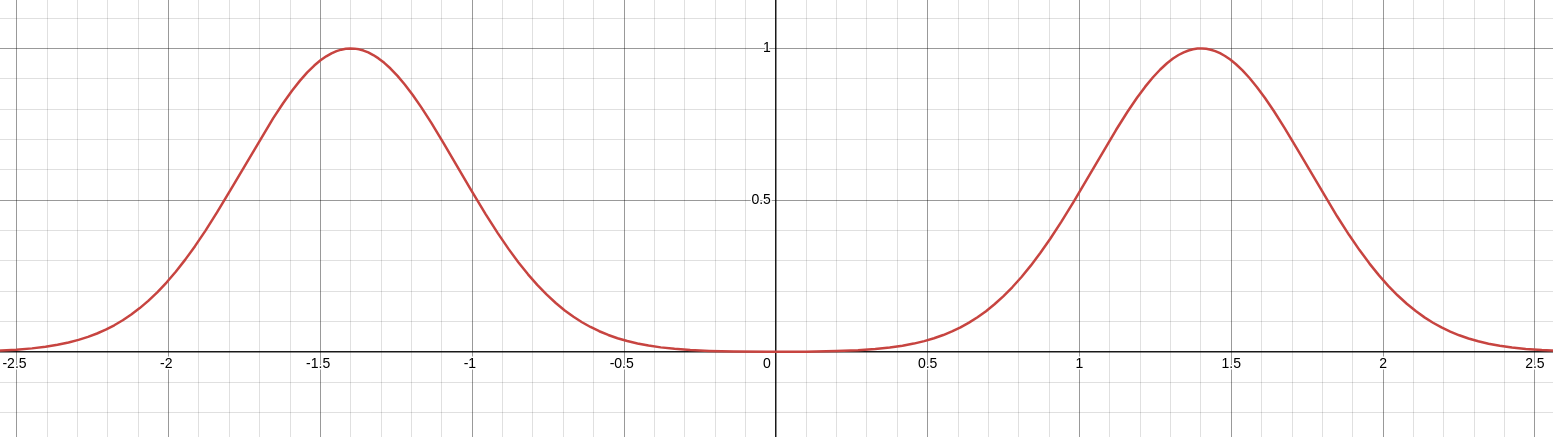
\includegraphics[width=0.9\textwidth]{fig/densi_spec_sym}
	\caption{Exemple de densité spectrale d'un signal réel ESP A 1,4}
	\label{fig:densi_spec_sym}
\end{figure}
\\
Même problème avec la covariance qui sera toujours nulle pour les signaux réels. De là en conclure que la fréquence instantanée de n'importe quel signal réel est toujours décorrélée du temps serait, pour le moins, insatisfaisant.
\\

Pour résoudre ces problèmes, il suffirait de ne conserver que la partie positive du spectre du signal. On s'intéresserait alors au signal transformée $\SA{x}$ tel que :
\[\mathcal{F}\big[\SA{x}\big] = 2\one_{\R^+}\fou{x}\]
où $\one_E$ est la fonction indicatrice sur l'ensemble $E$ et où le facteur 2 permet de conserver l'énergie du signal.
Avec la transformée de Fourier inverse, ce nouveau signal s'écrit alors :
\[\SA{x} = \mathcal{F}^{-1}\big[ 2\one_{\R^+}\fou{x} \big] = 2 \mathcal{F}^{-1}\big[\one_{\R^+}\big] * x\]
La transformée inverse de cette indicatrice (qui n'est autre que la fonction de Heavyside) n'est pas définie au sens classique, mais l'est au sens des distributions. Pour l'écrire, on introduit la distribution suivante :

\begin{definition}[Transformée en SA et de Hilbert]\label{def:transfo_sa&hilbert}
	On définie alors la \emph{transformée en signal analytique} (SA) de tout signal $x$ par l'application :
	\begin{equation}\label{eq:transfo_SA}
		\SA{x} = \sa{x} \defeq 2 x*\mathcal{F}^{-1}\big[\one_{\R^+}\big] :\ \begin{aligned} 
			\R \quad &\lr\qquad\quad \C \\	
			t\quad &\longmapsto\ x(t) + \frac{i}{\pi}\fint_\R \frac{x(s)}{t-s}ds
		\end{aligned}
	\end{equation}
	Par construction, on a bien $\mathcal{F}\big[\SA{x}\big] = 2\one_{\R^+}\fou{x}$, et on dira plus généralement de tout signal dont le spectre est réel positif que c'est un \emph{signal analytique}.
	\\
	L'intégral à droite de \eqref{eq:transfo_SA} est appelle \emph{transformée de Hilbert} du signal. Elle est notée :
	\begin{equation}\label{eq:transfo_Hilb}
		\mathcal{H}[x] :\ \begin{aligned} 
			\R \quad &\lr\qquad\quad \C \\	
			t\quad &\longmapsto\ \frac{1}{\pi}\fint_\R \frac{x(s)}{t-s}ds =  \frac{1}{\pi}\left(\vpC\right)*x
		\end{aligned}
	\end{equation}
\end{definition}

Par souci de commodité, plutôt que redéfinir tout le vocabulaire développé plus haut (fréquence moyenne, temps moyen, \etc) pour les signaux réel via la transformation $\mathcal{A}$, dans la suite du mémoire on travaillera directement avec $\SA{x}$. %^(et on verra que c'est essentiel).
\\



\subsubsection{Interprétabilité des signaux analytiques}\label{subsec:Bedrisan&AM-FM}

Dans les cas des signaux réels, la transformée de Hilbert est à valeur dans $\R$. Aussi, la transformée $\SA{x}$ à pour partie réelle $x$ et pour partie imaginaire $\mathcal{H}[x]$. Sous forme exponentielle, cela donne :
\[\SA{x}(t) = a(t)e^{i\phi(t)}\quad \Lr\quad \left\{\begin{aligned}x(t) &= a(t) \cos\phi(t) \\\mathcal{H}[x](t) &= a(t) \sin\phi(t)
\end{aligned}\right.\]
On obtient alors on décomposition de $x$ en une paire $(a,\phi)$ telle que discuté plus haut.

\begin{definition}[Amplitude et phase instantanée]\label{def:ampli&phase_instant}
	On définie ainsi l'\emph{amplitude instantanée} $a_x$ et la \emph{phase instantanée} $\phi_x$  de tout signal $x$ comme étant respectivement l'amplitude et la phase de $\SA{x}$ :
	\begin{align}\label{eq:ampli&phase_cano}
		a_x &= \big|\SA{x}\big|   &   \phi_x &= \arg\big(\SA{x}\big)
	\end{align}
\end{definition}

\begin{remarque}
	Il est important de noter que si un signal est présenté sous la forme  $\ x=a\cos\phi$, rien n'implique que $a$ et $\phi$ corresponde à l'amplitude et la phase instantanée du signal. Si ce n'est pas le cas, c'est que cette décomposition n'était ``pas la bonne'' en cela qu'elles ne s’interprètent pas comme l'on aimerait.
\end{remarque}

Pour comprendre comment cette transformation ``sélectionne'' la fréquence instantanée, détaillons le cas où $x$ s'écrit comme produit de deux signaux pures (\cref{fig:exemple_tSA_1/2}) :
\[x(t) = \cos (2\pi\nu_1t)\cos (2\pi\nu_2t)\]
\\
On montre sans mal\footnote{\itshape
	$\fou{x}$ est donné par 4 Diracs, en ne gardant que ce non nul sur $\R^+$ on obtient le spectre de $\SA{x}$ et il reste plus qu'à inverser la transformée de Fourier.}
que si $\nu_1\geq\nu_2$, alors la transformée en SA de $x$ s'écrit :
\[\SA{x} = \cos \left(2\pi\nu_2 t\right) e^{2\i\pi\nu_1 t}\]

\begin{figure}[h]\centering
	%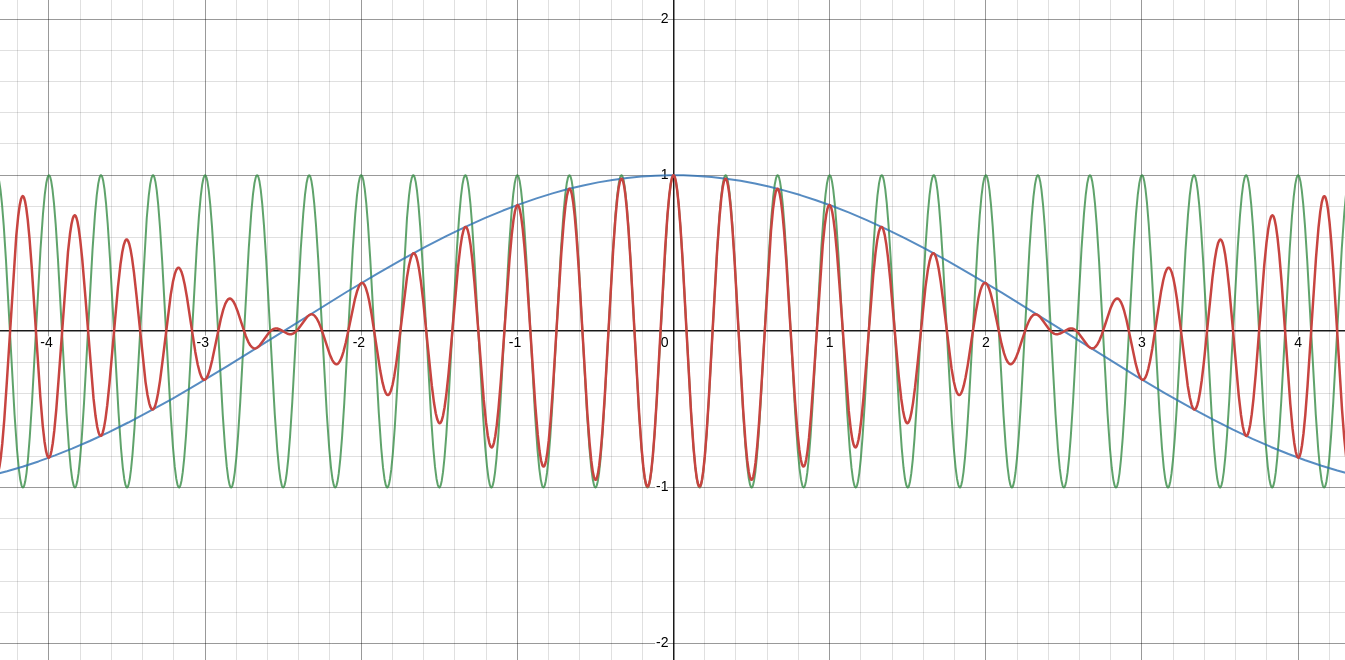
\includegraphics[width=0.48\textwidth]{fig/ex SA - 11.png}\hfill
	%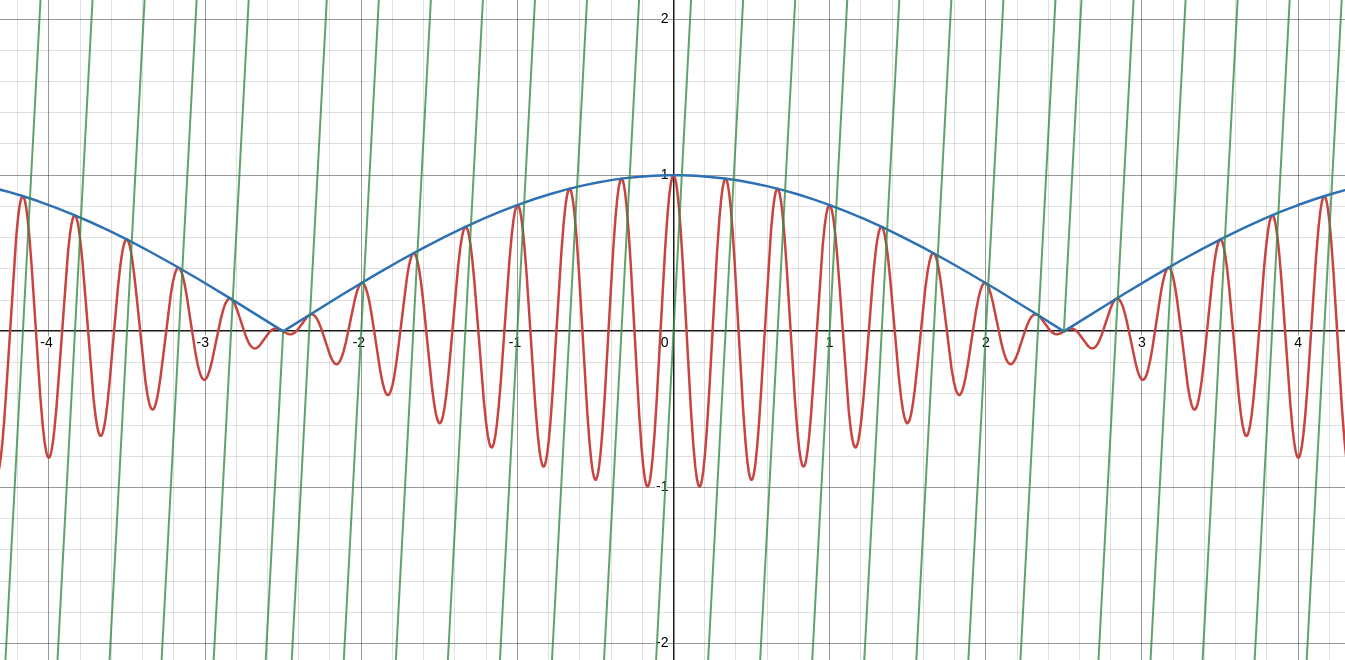
\includegraphics[width=0.48\textwidth]{fig/ex SA - 12.png}
	\caption{Représentation graphique du signal $x$ (rouge) avec $\nu_1=3$ et $\nu_2=0.1$. Sur l'image de gauche, avec signaux de fréquences pures (bleu et vert). Sur l'image de droite, avec son amplitude (bleu) et sa phase instantanée (vert). Les discontinuités de la phase sont dû à l'arrondi à $2\pi$  près de l'argument de $\SA{x}$ et à la façon dont il est calculé lorsque le signal s'annule (mise à 0). Voir \href{https://www.desmos.com/calculator/gcedcdfkhr}{ici} pour un graphique dynamique.}
	\label{fig:exemple_tSA_1/2}
\end{figure}
\noindent
Le signal $\SA{x}$ n'est ici pas sous forme exponentielle à proprement parler puisque le cosinus peut être négatif (pour s'y ramener, il suffit de passer le cos en valeur absolue et d'ajouter $\pi$ à l'argument lorsque nécessaire) mais l’avantage de cette forme est qu'elle fait clairement apparaître les fréquences $\nu_{1,2}$. En particulier, la fréquence instantanée du signal est la plus grandes des deux fréquences $\nu_1$ et $\nu_2$. La plus petite, elle, se retrouve dans l'amplitude. 
\\
Ce résultat est rassurant en cela qu'il est plus naturel de voir le cosinus de basse fréquence comme modulant celui de haute fréquence que l'inverse comme on le voit sur la première image de la figure \ref{fig:exemple_tSA_1/2}. 
\\
Aussi, en mettant les hautes fréquences du signal dans la fréquence instantanée, on s'assure de limiter les variations de l'amplitude. Cela apporte bien plus de contrainte en terme de décomposition $(a_x,\phi_x)$, en cela qui si l'inverse étant vrai, alors toute les fréquences pourrait être envoyé dans l'amplitude, ce qui laisserait la phase invariante.
\\

Cela étant dit, lorsque l'on fait varier $\nu_1$ et $\nu_2$, le résultat n'est pas toujours si intuitif. C'est notamment le cas lorsque les deux deviennent de plus en plus proche :

\begin{figure}[h]\centering
	%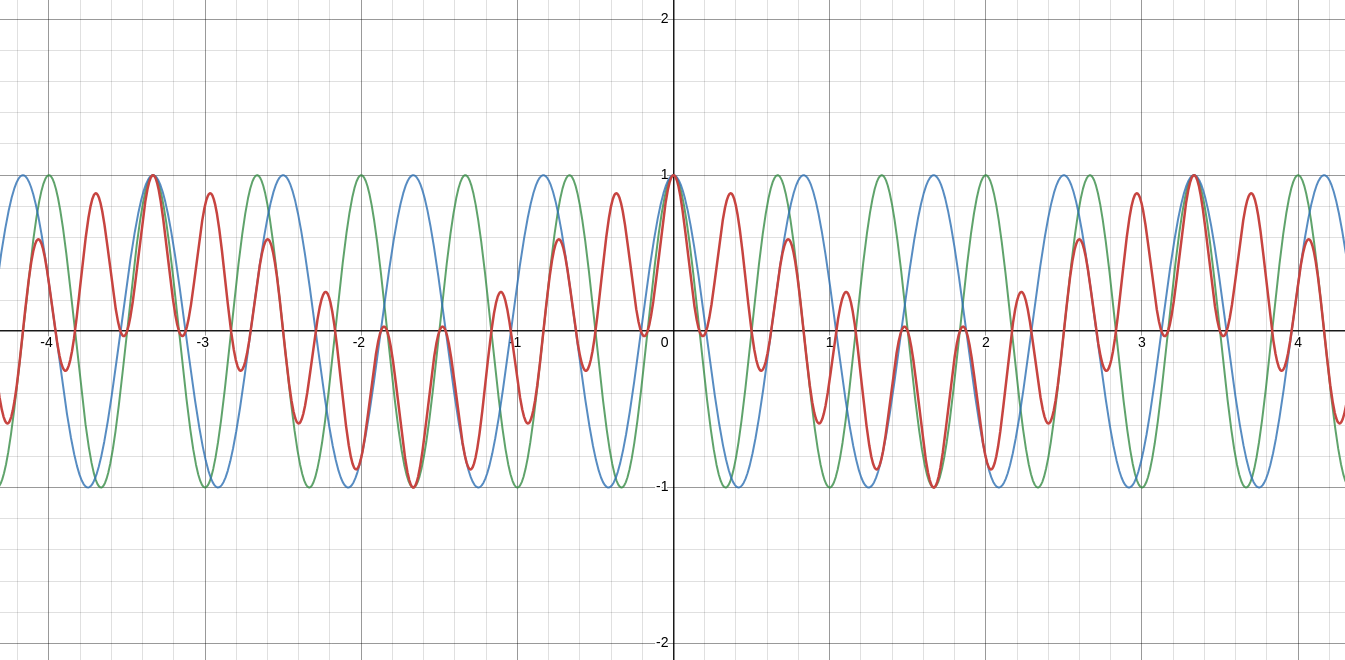
\includegraphics[width=0.48\textwidth]{fig/ex SA - 21.png}\hfill
	%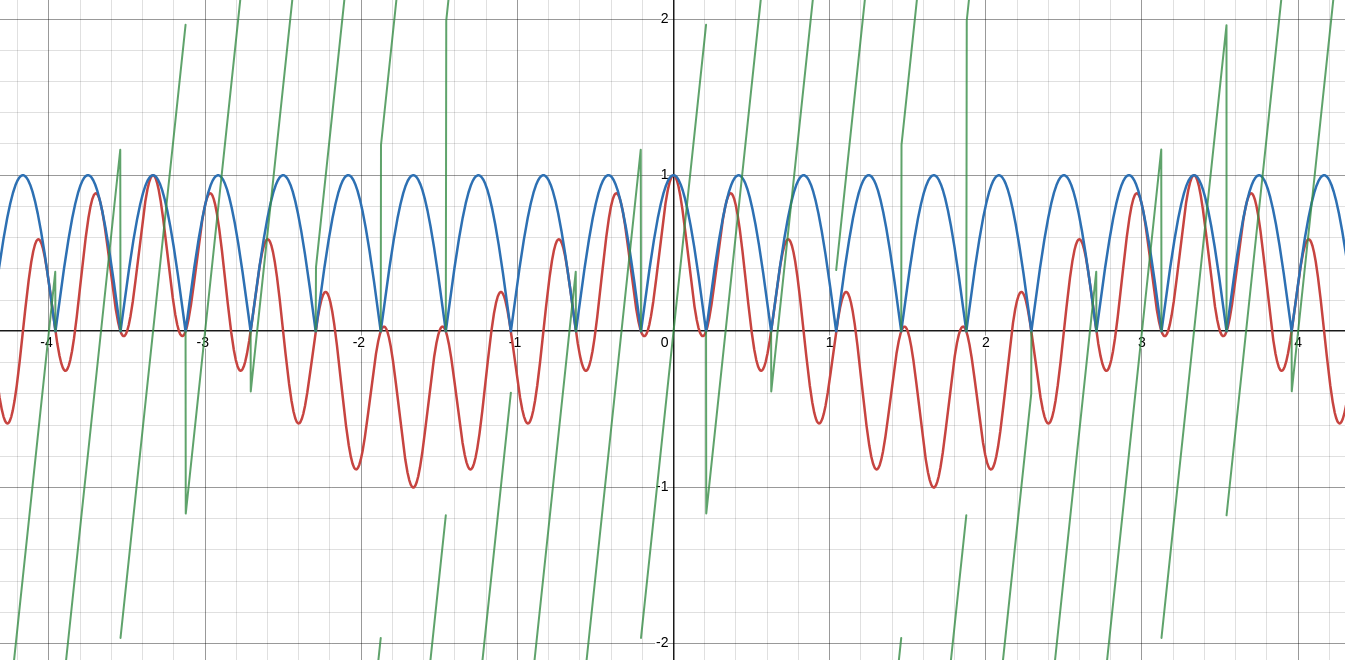
\includegraphics[width=0.48\textwidth]{fig/ex SA - 22.png}
	\caption{Idem que pour la figure \ref{fig:exemple_tSA_1/2} précédente, avec cette fois $\nu_1=1.5$ et $\nu_2=1.3$.}
	\label{fig:exemple_tSA_2/2}
\end{figure}

Pour comprendre pourquoi l'amplitude ne fait pas ce qu'on attendrait d'elle, on introduit le théorème de Bedrosian :

\begin{theoreme}[de Bedrosian]\label{theo:2Bedrosian}
	Dans sa formulation la plus générale, le théorème de Bedrosian énonce que donnée si deux fonctions $f,g\in L^2(\R)$ sont telles l'une des trois assertions suivantes est vraie :
	\newline
	\begin{itemize}%[label=\textit{\arabic*}. ]
		
		\item $\exists \lambda\in\R^+\ |\ \supp \fou{f} \subset [-\lambda, +\infty[,\ \supp \fou{g} \subset [\lambda, +\infty[$\label{item:1condi_theo2Bedrosian}
		
		\item $\exists \lambda\in\R^+\ |\ \supp \fou{f} \subset ]-\infty, \lambda],\ \supp \fou{g} \subset ]-\infty,-\lambda]$ \label{item:2condi_theo2Bedrosian}
		
		\item $\exists (\lambda_1,\lambda_2)\in \R^+\times\R^+ \setminus\{(0,0)\}\ |\ \supp \fou{f} \subset [-\lambda_1, \lambda_2],\ \supp \fou{g} \subset \R\setminus[-\lambda_2,\lambda_1]$
		
	\end{itemize}
	alors la transformée de Hilbert de leur produit est donnée par la formule (voir \cite{wang_simple_2009} pour une démonstration) :
	\begin{equation}\label{eq:2Bedrosian}
		\hilb{fg} = f\hilb{g}
	\end{equation}
\end{theoreme}

Dans le cas d'un signal réel, suivant la \cref{def:ampli&phase_instant} on peut écrire $\ x=a_x\cos\circ\phi_x$.
Comme $a_x$ et $\phi_x$ sont réelles, seule la deuxième condition du théorème de Bedrosian peut être satisfaite pour peu que $\lambda_1=\lambda_2$. Ainsi :

\begin{corollaire}\label{coro:AM-FM}
	Toujours avec les même notations, si $a_x\in L^2(\R)$, $\cos\phi_x\in L^2(\R)$ et qu'il existe $\lambda\in\R^{+_*}$ tel que :
	\[\supp \Fou{a_x} \subset [-\lambda, \lambda],\quad \supp \Fou{\cos\phi_x} \subset \R\setminus[-\lambda,\lambda]\]
	Alors on a :
	\begin{align*}
		\hilb{x} &= a_x\hilb{\cos \phi_x}  &  \qquad\qquad&\text{et si }a_x(t)\neq 0,  &  \hilb{\cos \phi_x}(t) = \sin\phi_x(t)
	\end{align*}
\end{corollaire}

Dans ce cas, 




\subsection{Généralisation aux signaux multivariés}\label{sec:sign_multivar}

\begin{definition}[Signal multivarié]\label{def:signal_multivar}
	Un \emph{signal multivarié}, ou \emph{$n-$varié}, est un vecteur composé de $n\in\N^*$ signaux $x_i$. Si $n=2$, alors on parle de signal \emph{bivarié}.
	\\
	Dans la continuité de ce qui à été dit dans la \cref{subsec:transfo_SA}, dans le cas des signaux réels, on s'intéressera au vecteur composé des transformées en SA (eq. \ref{eq:transfo_SA}, déf. \ref{def:transfo_sa&hilbert}) des $x_i$.
	\textbf{Au moins dans toute cette \namecref{sec:sign_multivar}}, un tel signal sera noté :
	\[\sa{x}(t)\ :\quad \begin{aligned} 
		\R\quad &\lr\qquad \C^n \\t\quad &\longmapsto\ \begin{pmatrix} \mathcal{A}[x_1] \\ 
			\mathcal{A}[x_2] \\ \vdots \\ \mathcal{A}[x_n] \end{pmatrix}
	\end{aligned} \]
	On supposera que chaque composante $x_i$ de $\bf{x}$ aura autant de régularité et de condition d'intégrabilité que nécessaire \textbf{(il vaudra préciser lesquelles à un moment)}.
\end{definition}

Le fait que $\bf{x}$ soit à valeur dans $\C^n$ impose un choix naturel de d'amplitude instantanée : sa norme. L'on notera alors dans tout la suite (sauf précision) :
\[\forall t\in\R,\qquad 
\bf{x}(t) = a(t)\begin{pmatrix} a_1(t)e^{i\phi_1(t)} \\ a_2(t)e^{i\phi_2(t)} \\ \vdots \\ a_n(t)e^{i\phi_n(t)}
\end{pmatrix} \qquad\text{ avec }\qquad \big\|(a_i)_{1\leq i\leq n}\big\|=1,\quad a\geq 0
%a(t)e^{i\phi(t)}\begin{pmatrix} a_1(t)e^{i\psi_1(t)} \\ a_2(t)e^{i\psi_2(t)} \\ \vdots \\ a_n(t)e^{i\psi_n(t)}\end{pmatrix}
\]
\\
Le choix de la phase instantanée, en revanche, n'est pas plus commode. Si l'on cherche à écrire $\bf{x}$ sous la forme :
\[a(t)e^{i\phi(t)}\begin{pmatrix} a_1(t)e^{i\psi_1(t)} \\ a_2(t)e^{i\psi_2(t)} \\ \vdots \\ a_n(t)e^{i\psi_n(t)}
\end{pmatrix}\]
alors n'importe quel choix de $\phi$ est valable, il suffit que $\ \psi_i = \phi_i-\phi$.




\subsubsection{Phase et fréquence instantanée de signal multivarié }\label{subsec:param_instant_nvar}

Afin de contraindre ce choix, on s'inspire propriétés de la phase instantanée vu plus tôt pour en déduire deux approches :
\begin{itemize}
	\item D'une part, l'espérance de la fréquence instantanée (ici vu comme dérivée à $2\pi$ près de la phase\footnote{\itshape
		La pertinance de cette définition dans le cas multivarié sera discuté plus loin})
	doit donnée la fréquence moyenne au sens de Fourier, eq. \eqref{eq:esp_freq}.
	
	\item D'autre part, les conditions d'interprétation de la décomposition $(a_x,\phi_x)$, \cref{theo:2Bedrosian}, exige que les hautes fréquences du signal se retrouve dans la phase.
\end{itemize}

Pour cela on introduit les notations utiles au cas multivarié :
\begin{definition}[densité d’énergie]\label{def:densi_dE-mv}
	Étant donné un signal multivarié $\bf{x}=(x_i)_{1\leq i\leq n}$, les densités d'énergie de chaque composante $x_i$  sont notées :
	\begin{align}\label{eq:densi_dEi}
		\densit_i\ &:\quad \begin{aligned}\R\ &\lr\quad \R^+ \\ t\ &\longmapsto\ \big|x_i(t)\big|^2 = a(t)^2 a_i(t)^2 \end{aligned}  
		&
		\densis_i\ &:\quad \begin{aligned}\R\ &\lr\quad \R^+ \\ \nu\ &\longmapsto\ \big|\fou{x}_i(\nu)\big|^2 \end{aligned}
	\end{align}
	Et les densités d'énergies associées au signal $\bf{x}$ complet :
	\begin{align}\label{eq:densi_dE-mv}
		\densit\ &:\quad \begin{aligned}\R\ &\lr\quad \R^+ \\ t\ &\longmapsto\ \big\|\bf{x}(t)\big\|^2 = \sum_{i=1}^n \densit_i(t) \end{aligned}  
		&
		\densis\ &:\quad \begin{aligned}\R\ &\lr\quad \R^+ \\ \nu\ &\longmapsto\ \big\|\fou{\bf{x}}(\nu)\big\|^2 = \sum_{i=1}^n \densis_i(t) \end{aligned}	
	\end{align}
\end{definition}

La première approche, inspiré de \cite{cano_mathematical_2022} consiste donc de reprendre le ``calculation trick'' \eqref{eq:moment_f}, pour en déduire la fréquence moyenne
\begin{align*}
	\esp[\densis]{\nu} = \int_\R \nu\densis(\nu)d\nu &= \int_\R \nu\sum_{i=1}^n \densis_i(\nu) d\nu \\
	&= \sum_{i=1}^n\esp[\densis_i]{\nu} \\
	&= \sum_{i=1}^n\frac{1}{2\pi}\int_\R \phi_i'(t)\densit_i(t)dt \\
	&= \frac{1}{2\pi}\int_\R a(t)^2\sum_{i=1}^n\phi_i'(t)a_i(t)^2 dt 
	\\ &= \frac{1}{2\pi} \esp[\densit]{\sum_{i=1}^n \phi_i'{a_i}^2}
\end{align*}
\\
Ce qui mène à une première définition de la phase instantanée :
\begin{equation}\label{eq:phas_inst_v1}
	\phi = \int \sum_{i=1}^n \phi_i'(s){a_i}(s)^2ds 
	= \sum_{i=1}^n \int \phi_i'(s){a_i}(s)^2ds 
	%= \sum_{i=1}^n \esp[\nicefrac{\densit_i}{\densit}]{\phi_i'}
\end{equation}
\\

La seconde approche, fortement inspirée par les travaux de Lilly \& Olhede  \cite{lilly_analysis_2012}, se base sur la discussion autour du théorème Bedrisan sur la séparation haute-basse fréquence du signal $\bf{x}$ (\cref{subsec:Bedrisan&AM-FM}). Pour cela, l'on commence par faire apparaître la phase $\phi$ --- pour l'instant inconnue --- en écrivant $\bf{x}$ sous la forme :
\[\forall t\in\R,\qquad \bf{x}(t) = e^{i\phi(t)} e^{-i\phi(t)} \bf{x}(t) \defeq e^{i\phi(t)} \Tilde{\bf{x}}(t)\]
\\
Si $\phi$ est bien choisie, alors $\Tilde{\bf{x}}$ contient les informations associées à l'amplitude et la polarisation de $\bf{x}$. Or, la phase doit contenir les hautes fréquences du signal. 
Pour s'en assurer on demande, à l'inverse, que les basses fréquences du signal soit données par $\Tilde{\bf{x}}$ en limitant ces variations. En clair, $\phi$ doit être choisi de sorte à minimiser la dérivée $\Tilde{\bf{x}}'$ :
\[\forall t\in\R,\qquad \phi(t) = \argmin{\alpha(t)}{\big\|\Tilde{\bf{x}}'(t)\big\|_2}^2 = \argmin{\alpha(t)}{\Big\|e^{-i\alpha}\big(\bf{x}' - i\alpha'\bf{x}\big)\Big\|_2}^2 = \argmin{\alpha(t)}{\big\|\bf{x}' - i\alpha'\bf{x}\big\|_2}^2\]
\\
La contrainte ne dépendant que de la dérivée $\alpha'$, on se ramène à :
\[\min_{\alpha(t)}{\|\Tilde{\bf{x}}'(t)\|_2}^2 = \min_{\alpha'(t)}{\big\|\bf{x}'(t) - \alpha'(t) \bf{x}(t)\big\|_2}^2\]
\\
En rappelant que $\frac{d}{dx}{\big\|f(x)\big\|_2}^2 = 2\Re e\big\langle f(x), f'(x)\big\rangle$, il vient que ce minimum\footnote{\itshape
	L'extremum obtenu est l'unique minimum puisque $t\longmapsto \|at + b\|^2$ est strictement convexe pour $a\neq0$.}
est atteint par $\phi'(t)$ à condition que :
\begin{align*}
	\frac{d}{d\phi'}{\big\| \bf{x}' - i\phi' \bf{x}\big\|_2}^2 = 0 \quad \Llr\quad
	0 &= 2\Re e\left\langle  \bf{x}' - i\phi' \bf{x} ,  \frac{d}{d\phi'}\big(\bf{x}' - i\phi' \bf{x}\big)\right\rangle \\
	&= 2\Re e\big\langle  \bf{x}' - i\phi' \bf{x} ,  - i \bf{x}\big\rangle \\
	&= 2\Re e\Big(i\big\langle  \bf{x}' ,  \bf{x}\big\rangle\Big) + 2\phi'\Re e\big\langle   \bf{x} ,  \bf{x}\big\rangle\\
	&= -2\Im m\big\langle  \bf{x}' ,  \bf{x}\big\rangle + 2\phi'{\| \bf{x}\|_2}^2
\end{align*}
Ainsi :
\begin{align}\label{eq:phas_inst_v2}
	\phi' &= \frac{\Im m\big\langle  \bf{x}' ,  \bf{x}\big\rangle}{{\| \bf{x}\|_2}^2} = \frac{-\Im m\big\langle  \bf{x},  \bf{x}'\big\rangle}{{\| \bf{x}\|_2}^2}  &  &\text{et}  &  \phi &= -\Im m\int \frac{\big\langle \bf{x}(s) , \bf{x}'(s) \big\rangle}{\|\bf{x}(s)\|^2} ds
\end{align}
\\
Ce qui, sous forme exponentiel, se réécrit :
\begin{align*}
	-\Im m\frac{\big\langle \bf{x}(t) , \bf{x}'(t) \big\rangle}{\|\bf{x}(t)\|^2} &= -\Im m\frac{1}{a(t)^2} \sum_{i=1}^n a(t)a_i(t)e^{i\phi_i(t)}\congu{\Big( \big(aa_i\big)'(t) +a(t)a_i(t)i\phi_i'(t)\Big)e^{i\phi_i(t)}} \\
	&= -\Im m\frac{1}{a(t)^2} \sum_{i=1}^n a(t)a_i(t)\big(aa_i\big)'(t) -ia(t)^2a_i(t)^2\phi_i'(t) \\
	&= -\frac{1}{a(t)^2} \sum_{i=1}^n -a(t)^2a_i(t)^2 \phi_i'(t) \\
	&= \sum_{i=1}^n a_i(t)^2 \phi_i'(t)
\end{align*}
Soit la même expression que \eqref{eq:phas_inst_v1} obtenue par le premier raisonnement.
\\
\begin{remarque}[Notation à reprendre ($aa_i$)]
	Toujours avec les mêmes notations, une conséquence de l'\cref{eq:phas_inst_v2} est que les fréquences $\psi_i$ restantes sont de moyenne nulle dans le sens où :
	\begin{equation}\label{eq:sum_esp_null}
		\sum_{i=1}^n \int \psi_i'(s){a_i}(s)^2ds =0
	\end{equation}
	Moralement, ca revient juste à dire qu'en définissant $\phi$ suivant Lilly, on a ôté au $\psi_i$ la phase moyenne pondérée et donc, tout naturellement, les nouvelles phase individuelles $\psi_i$ sont centrés (à la même pondération près). Cela revient peut ou prou à la première \cref{eq:phas_inst_v1}.
	\\
	Pour le montrer, il suffit de refaire le calcul de la phase instantanée :
	\begin{align*}
		\big\langle \bf{x}(t) \,|\, \dot{\bf{x}}(t) \big\rangle &= \Big\langle \Big(a_i(t)e^{i(\phi(t)+\psi_i(t))}\Big)_i \,\Big|\, \Big(\big(a_i'(t)+i\big( \phi(t)+\psi_i(t) \big)a_i(t)\big)e^{i(\phi(t)+\psi_i(t))}\Big)_i \Big\rangle \\
		&= \sum_i a_i(t) \Big(a_i'(t)-i\big(\phi'(t) + \psi_i'(t)\big)a_i(t)\Big) \\
		&= \sum_i a_i(t)a_i'(t)-i\sum_i \big(\phi'(t) + \psi_i'(t)\big)a_i(t)^2 \\
		&= \sum_i a_i(t)a_i'(t)-i \phi'(t)\sum_ia_i(t)^2  - i\sum_i \psi_i'(t)a_i(t)^2 \\
		&= \sum_i a_i(t)a_i'(t)-i \phi'(t)\big\|a(t)\big\|^2  - i\sum_i \psi_i'(t)a_i(t)^2
	\end{align*}
	\\
	Ce qui mène à :
	\begin{align*}
		\phased(\bf{x},t_0,t) &= \int_{t_0}^t \frac{\varphi'(s)\big\|a(s)\big\|^2}{\big\|a(s)\big\|^2} ds  + \sum_i\int_{t_0}^t \frac{\varphi_i'(s)a_i(s)^2}{\big\|a(s)\big\|^2} ds \\
		&=\phased(\bf{x},t_0,t)  + = \sum_{i=1}^n \int \psi_i'(s){a_i}(s)^2ds 
	\end{align*}
\end{remarque}




\subsubsection{Apparition de la phase géométrique}\label{subsub:intro_phaseg}





\begin{annexe}

\section{Complément sur l'analyse temps-fréquence} 

\subsection{Un bon moment...}\label{ann:integ_trick}

Pour montrer les formules de la \cref{prop:mom_freq}, on commence par montrer ce que Cohen \cite{cohen_time_1995} appelle les  :

\begin{proposition}[``Calculation tricks''] \label{prop:integ_trick}
	Si le signal est $n$ fois dérivable et que la densité d’énergie spectrale associée $\densis$ admet un moment d'ordre $n$, alors ce moment est donnée par la formule :
	\begin{equation}\label{eq:moment_f}
		\forall n\in\N,\qquad \esp[\densis]{\nu^n} = \left(\frac{i}{2 \pi}\right)^n  \int_\R x(t) \frac{d^n}{dt^n} \congu{x(t)} dt = \left(\frac{i}{2 \pi}\right)^n  \left\langle x, \frac{d^n}{dt^n}x\right\rangle
	\end{equation}
	\\
	Avec les hypothèses analogues, les moments de $\densit$ s'écrivent :
	\begin{equation}\label{eq:moment_t}
		\forall n\in\N,\qquad \esp[\densit]{t^n} = \left(\frac{1}{2i \pi}\right)^n  \int_\R \fou{x}(\nu) \frac{d^n}{dt^n} \congu{\fou{x}(\nu)} dt = \left(\frac{1}{2i \pi}\right)^n  \left\langle \fou{x}, \frac{d^n}{d\nu^n}\fou{x}\right\rangle
	\end{equation}
\end{proposition}


\begin{demo}[de la \cref{prop:integ_trick}]
	\`A supposer que les intégrales existes et que le théorème de Fubini s'applique, on a $\forall n\in\N$ :
	\begin{align*}
		\esp[\densis]{\nu^n} = \int_\R \nu^n\densis(\nu) d\nu &= \int_\R \nu^n \fou{x}(\nu)\congu{\fou{x}(\nu)} d\nu \\
		&= \int_\R \nu^n \int_\R x(t)e^{-2i \pi \nu t} dt \int_\R \congu{x(t')}e^{2i \pi \nu t'} dt' d\nu \\
		&= \int_\R \int_\R x(t) \congu{x(t')} \int_\R \nu^n e^{-2i \pi \nu (t-t')} d\nu dt dt' 
	\end{align*}
	Ici, on remarque que :
	\begin{align*}
		\nu^n e^{-2i \pi \nu (t-t')} &= \nu^{n-1}\frac{1}{-2i \pi}\frac{d}{dt}e^{-2i \pi \nu(t-t')} \\
		&= \nu^{n-2}\frac{1}{(-2i \pi)^2}\frac{d^2}{dt^2}e^{-2i \pi \nu(t-t')} \\
		&\ \vdots \\
		&= \frac{1}{(-2i \pi)^n}\frac{d^n}{dt^n}e^{-2i \pi \nu(t-t')}
	\end{align*}
	\\
	
	Ce qui permet, en jouant sur les ordres d'intégrations et les propriétés du Dirac, d'obtenir :
	\begin{align*}
		\esp[\densis]{\nu^n} &= \int_\R \int_\R x(t) \congu{x(t')} \int_\R \nu^n e^{-2i \pi \nu (t-t')} d\nu\, dt\, dt' \\
		&= \int_\R \int_\R x(t) \congu{x(t')} \int_\R \frac{1}{(-2i \pi)^n}\frac{d^n}{dt^n}e^{-2i \pi \nu(t-t')} d\nu\, dt\, dt' \\
		&= \frac{1}{(-2i \pi)^n} \int_\R \int_\R x(t) \congu{x(t')} \frac{d^n}{dt^n}\int_\R e^{-2i \pi \nu(t-t')} d\nu\, dt\, dt' \\
		&= \left(\frac{1}{-2i \pi}\right)^n \int_\R \int_\R x(t) \congu{x(t')} \frac{d^n}{dt^n}\mathcal{F}\big[1\big](t-t') dt\, dt' \\
		&= \left(\frac{i}{2 \pi}\right)^n \int_\R \int_\R x(t) \congu{x(t')} \frac{d^n}{dt^n}\delta(t-t') dt\, dt' \\
		&= \left(\frac{i}{2 \pi}\right)^n \int_\R x(t) \int_\R \congu{x(t')} \frac{d^n}{dt^n}\delta(t-t') dt' dt \\
		&= \left(\frac{i}{2 \pi}\right)^n  \int_\R x(t) \frac{d^n}{dt^n}  \congu{x(t)} dt
	\end{align*}
	%	... a moins que :
\end{demo}

\begin{demo}[de l'\cref{eq:esp_freq}, \cref{prop:mom_freq}]
	Avec le hypothèses de la \cref{prop:integ_trick} précédente, on a :
	\begin{align*}
		\esp[\densis]{\nu} = \frac{i}{2\pi} \densit(t) \int_\R x(t) \congu{x'(t)} dt &= \frac{i}{2\pi}\int_\R a(t)e^{i\phi(t)}\congu{\big( a'(t)e^{i\phi(t)}+ ia(t)\phi'(t)e^{i\phi(t)} \big)} dt \\
		&= \frac{i}{2\pi}\int_\R a(t)e^{i\phi(t)}\big( a'(t)e^{-i\phi(t)} -ia(t)\phi'(t)e^{-i\phi(t)} \big) dt \\
		&= \frac{i}{2\pi}\int_\R a(t)\big( a'(t)- ia(t)\phi'(t)\big) dt \\
		&= \frac{i}{2\pi}\int_\R a'(t)a(t) dt + \int_\R  \frac{1}{2\pi}\phi'(t)a(t)^2 dt \\
	\end{align*}
	On peut se convaincre que le premier terme doit être nul car l'espérance doit être réelle. On peut s'en assurer par le calcul en notant que c'est l’inégale d'une dérivée :
	\[\int_\R a'(t)a(t) dt = \frac{1}{2} \int_\R \big(a^2\big)'(t) dt = \frac{1}{2}\densit(t)\Big|_{-\infty}^{+\infty} = 0\]
	Ce qui donne bien :
	\[\esp[\densis]{\nu} = \frac{i}{2\pi}\int_\R a'(t)a(t) dt + \int_\R  \frac{1}{2\pi}\phi'(t)a(t)^2 dt = \frac{1}{2\pi}\int_\R \phi'(t)\densit(t) dt\]
\end{demo}

\begin{demo}[de l'\cref{eq:var_freq}, \cref{prop:mom_freq}]
	à démo comme PNL
\end{demo}

	
\subsection{Transformée inverse de la fonction de Heaviside}

\begin{definition}[valeur principale de Cauchy]\label{def:vp&Hilb}
	On appelle \emph{valeur principale de Cauchy} la distribution, notée $\vpC$, telle que :
	\begin{equation}
		\begin{aligned}
			\forall \varphi\in\mathcal{S}(\R),\qquad 
			\left\langle \vpC, \varphi \right\rangle 
			= \fint_0^t \frac{\varphi(t)}{t}dt 
			&\defeq \lim_{\varepsilon\lr0^+} \int_{-\infty}^{-\varepsilon} \frac{\varphi(t)}{t}dt + \int_{+\varepsilon}^{+\infty} \frac{\varphi(t)}{t}dt \\
			&= \int_0^{+\infty} \frac{\varphi(t) - \varphi(-t)}{t}dt
		\end{aligned}
	\end{equation}
	Ici $\mathcal{S}(\R)$ est l’espace de Schwartz des fonctions $C^\infty$ à décroissance rapide et la limite en $\varepsilon$ assure que l'intégrale (impropre) converge bien. Sa valeur est également appelée \emph{valeur principale} de l'intégrale. 
\end{definition}

La distribution vp$\frac{1}{x}$ est la valeur principale de la fonction inverse dans le sens où son produit avec l'identité donne 1 $\big(\left\langle id_\R \times \vpC, \varphi \right\rangle = \left\langle \vpC, id_\R \times\varphi \right\rangle=1\big)$ mais avec des propriétés d'intégration supplémentaires. Entre autre :

\begin{propriete}\label{prop:fou2vp}
	La transformée de Fourier de la valeur principale de Cauchy est donnée, au sens des distributions, par :
	\begin{equation}
		\mathcal{F} \left[\vpC \right]= -i \pi\, \sign{} 
	\end{equation}
	On en déduit la transformée de Fourier inverse :
	\begin{equation}
		\mathcal{F}^{-1}\big[ 2\one_{\R^+} \big] = \mathcal{F}^{-1}\big[ 1 + \sign \big] = \delta + \frac{i}{\pi} \vpC
	\end{equation}
\end{propriete}

\begin{demo}
	juste pour le plaisir. Par définition, la transformée de Fourier de la valeur principale est telle que,\\ $\forall \varphi\in\mathcal{S}(\R)$ :
	\begin{align*}
		\left\langle \mathcal{F} \left(\vpC \right), \varphi \right\rangle = \left\langle \vpC, \hat{\varphi} \right\rangle 
		&= \fint_\R \frac{\hat{\varphi}(\nu)}{\nu} d\nu \\
		&= \int_0^{+\infty} \frac{\hat{\varphi}(\nu) - \hat{\varphi}(-\nu)}{\nu} d\nu \\
		&= \int_0^{+\infty} \frac{1}{\nu} \left( \int_\R\varphi(t)e^{-2i\pi \nu t}dt - \int_\R\varphi(t)e^{2i\pi \nu t}dt \right)d\nu \\
		&= \int_0^{+\infty} \frac{1}{\nu}\int_\R\varphi(t)\big(e^{-2i\pi \nu t} - e^{2i\pi \nu t}\big)dt\, d\nu \\
		&= \int_0^{+\infty} \frac{1}{\nu}\int_\R-2i\varphi(t)\sin(2\pi \nu t)dt\, d\nu \\
		&= -2i\int_\R\varphi(t)\int_0^{+\infty} \frac{\sin(2\pi \nu t)}{\nu}d\nu\, dt
	\end{align*}
	En posant $u=2\pi\nu t\sign(t)$ (le signe de $t$ assure que l'on ait le même signe dans et hors du sin), on obtient :
	\begin{align*}
		\left\langle \mathcal{F} \left[\vpC \right], \varphi \right\rangle &= -2i\int_\R\varphi(t)\int_0^{+\infty} \sign(t)\frac{\sin(u)}{u}du\, dt \\
		&= -2i\int_\R\varphi(t)\frac{\pi}{2}\sign(t), dt \\
		&= \big\langle -i\pi\sign, \varphi \big\rangle
	\end{align*}
\end{demo}

\end{annexe}





\newpage

\listoffigures
\vfill
\lstlistoflistings
\vfill
%\listtheorems

\newpage

\bibliography{ref.bib}{}
\bibliographystyle{siam}
\end{document}